% 原书印刷页 1–4；按源页逐段重译，所有数学均为原生 LaTeX。
\sourcepage{1}
本讲义讨论如下问题。

\begin{statement}{定义 1.1\quad 最小二乘问题}
求 $\mathbf{x}^{*}$，使其为下列函数的一个局部极小点\footnotemark[1]：
\[
 F(\mathbf{x})=\frac12\sum_{i=1}^{m}\bigl(f_i(\mathbf{x})\bigr)^2,
\]
其中 $f_i:\R^n\to\R$，$i=1,\ldots,m$ 是给定的函数，且 $m\ge n$。
\end{statement}
\footnotetext[1]{定义 $F(\mathbf{x})$ 时引入的因子 $\tfrac12$ 不影响 $\mathbf{x}^{*}$。引入它是为了方便，见第~\pageref{src:18}~页。}
\setcounter{footnote}{1}

\begin{example}{1.1}
最小二乘问题的一个重要来源是数据拟合。例如，考虑下图所示的数据点 $(t_1,y_1),\allowbreak\ldots,\allowbreak(t_m,y_m)$。

\begin{figure}[H]
\centering
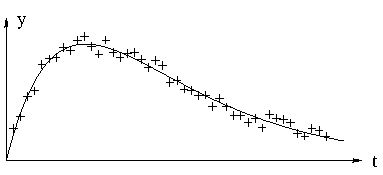
\includegraphics[width=0.67\linewidth]{assets/figures/fig-1-1.pdf}
\setcounter{figure}{0}
\caption{数据点 $\{(t_i,y_i)\}$（以 $+$ 标记）与模型 $M(\mathbf{x},t)$（以实线表示）。}
\label{fig:1.1}
\end{figure}
此外，给定一个拟合模型，
\[
 M(\mathbf{x},t)=x_3e^{x_1t}+x_4e^{x_2t}.
\]

\sourcepage{2}
该模型取决于参数 $\mathbf{x}=[x_1,x_2,x_3,x_4]^{\T}$。我们假定存在某个 $\mathbf{x}^{\dagger}$，使得
\[
 y_i=M(\mathbf{x}^{\dagger},t_i)+\varepsilon_i,
\]
其中 $\{\varepsilon_i\}$ 是数据纵坐标的（测量）误差，假定其表现如同“白噪声”。

对于任意选定的 $\mathbf{x}$，我们都可以计算残差
\[
\begin{aligned}
 f_i(\mathbf{x})&=y_i-M(\mathbf{x},t_i)\\
 &=y_i-x_3e^{x_1t_i}-x_4e^{x_2t_i},\qquad i=1,\ldots,m.
\end{aligned}
\]
对于最小二乘拟合，参数取为残差平方和的极小点 $\mathbf{x}^{*}$。可见，这是定义 1.1 所述形式的问题，其中 $n=4$。图~\ref{fig:1.1} 中的实线表示 $M(\mathbf{x}^{*},t)$ 的图像。
\end{example}

最小二乘问题是以下更一般问题的一种特殊形式：给定函数 $F:\R^n\to\R$，求使这个所谓的目标函数或代价函数取得最小值的自变量。

\begin{statement}{定义 1.2\quad 全局极小点}
给定 $F:\R^n\to\R$。求
\[
 \mathbf{x}^{+}=\operatorname*{arg\,min}_{\mathbf{x}}\{F(\mathbf{x})\}.
\]
\end{statement}

一般而言，这个问题很难求解。我们只介绍求解一个较简单问题的方法，即寻找 $F$ 的局部极小点：在某个区域内使 $F$ 取得最小值的自变量向量，该区域的大小由 $\delta$ 给定，其中 $\delta$ 是一个较小的正数。

\begin{statement}{定义 1.3\quad 局部极小点}
给定 $F:\R^n\to\R$。求 $\mathbf{x}^{*}$，使得
\[
 F(\mathbf{x}^{*})\le F(\mathbf{x})\qquad\text{当 }\norm{\mathbf{x}-\mathbf{x}^{*}}<\delta.
\]
\end{statement}

本章余下部分将讨论优化中的一些基本概念；第 2 章简要回顾为一般代价函数寻找局部极小点的方法。
\sourcepage{3}
更多细节参见 Frandsen 等（2004）。第 3 章给出专为最小二乘问题设计的方法。

我们假定代价函数 $F$ 可微，并且足够光滑，使以下泰勒展开成立\footnote{除非另有说明，$\norm{\cdot}$ 表示 2-范数，即 $\norm{\mathbf{h}}=\sqrt{h_1^2+\cdots+h_n^2}$。}：
\begin{equation}
 F(\mathbf{x}+\mathbf{h})=F(\mathbf{x})+\mathbf{h}^{\T}\mathbf{g}
 +\frac12\mathbf{h}^{\T}\mathbf{H}\mathbf{h}+O(\norm{\mathbf{h}}^3),
 \tag{1.4a}\label{eq:1.4a}
\end{equation}
其中 $\mathbf{g}$ 为梯度，
\begin{equation}
 \mathbf{g}\equiv \mathbf{F}'(\mathbf{x})=
 \begin{bmatrix}
  \dfrac{\partial F}{\partial x_1}(\mathbf{x})\\[1ex]
  \vdots\\[1ex]
  \dfrac{\partial F}{\partial x_n}(\mathbf{x})
 \end{bmatrix},
 \tag{1.4b}\label{eq:1.4b}
\end{equation}
而 $\mathbf{H}$ 为海森矩阵，
\begin{equation}
 \mathbf{H}\equiv \mathbf{F}''(\mathbf{x})=
 \left[\frac{\partial^2F}{\partial x_i\partial x_j}(\mathbf{x})\right].
 \tag{1.4c}\label{eq:1.4c}
\end{equation}

如果 $\mathbf{x}^{*}$ 是局部极小点，且 $\norm{\mathbf{h}}$ 足够小，那么就不可能找到一个点 $\mathbf{x}^{*}+\mathbf{h}$，使其 $F$ 值更小。将这一观察与式~\eqref{eq:1.4a} 结合，得到

\begin{statement}{定理 1.5\quad 局部极小点的必要条件}
如果 $\mathbf{x}^{*}$ 是局部极小点，则
\[
 \mathbf{g}^{*}\equiv \mathbf{F}'(\mathbf{x}^{*})=\mathbf{0}.
\]
\end{statement}

对于满足这一必要条件的自变量，我们使用一个专门的名称。

\begin{statement}{定义 1.6\quad 驻点}
如果
\[
 \mathbf{g}_{\mathrm{s}}\equiv \mathbf{F}'(\mathbf{x}_{\mathrm{s}})=\mathbf{0},
\]
则称 $\mathbf{x}_{\mathrm{s}}$ 为 $F$ 的一个驻点。
\end{statement}

\sourcepage{4}
因此，局部极小点也是驻点，但局部极大点同样也是驻点。既不是局部极大点、也不是局部极小点的驻点称为鞍点。为了判定一个给定的驻点是否为局部极小点，需要计入泰勒级数~\eqref{eq:1.4a} 中的二阶项。代入 $\mathbf{x}_{\mathrm{s}}$，可得
\begin{equation}
\begin{aligned}
 F(\mathbf{x}_{\mathrm{s}}+\mathbf{h})
 &=F(\mathbf{x}_{\mathrm{s}})+\frac12\mathbf{h}^{\T}\mathbf{H}_{\mathrm{s}}\mathbf{h}
   +O(\norm{\mathbf{h}}^3)\\
 &\hspace{1.5em}\text{其中 }\mathbf{H}_{\mathrm{s}}=\mathbf{F}''(\mathbf{x}_{\mathrm{s}}).
\end{aligned}
\tag{1.7}\label{eq:1.7}
\end{equation}

由海森矩阵的定义~\eqref{eq:1.4c} 可知，任意 $\mathbf{H}$ 都是对称矩阵。如果要求 $\mathbf{H}_{\mathrm{s}}$ 正定，那么它的特征值均大于某个数 $\delta>0$（见附录 A），并且
\[
 \mathbf{h}^{\T}\mathbf{H}_{\mathrm{s}}\mathbf{h}>\delta\norm{\mathbf{h}}^2.
\]
这表明，当 $\norm{\mathbf{h}}$ 足够小时，式~\eqref{eq:1.7} 右侧的第二项将支配第三项。而第二项是正的，因此得到

\begin{statement}{定理 1.8\quad 局部极小点的充分条件}
假设 $\mathbf{x}_{\mathrm{s}}$ 是一个驻点，且 $\mathbf{F}''(\mathbf{x}_{\mathrm{s}})$ 正定。则 $\mathbf{x}_{\mathrm{s}}$ 是一个局部极小点。
\end{statement}

如果 $\mathbf{H}_{\mathrm{s}}$ 负定，则 $\mathbf{x}_{\mathrm{s}}$ 是局部极大点。如果 $\mathbf{H}_{\mathrm{s}}$ 不定（即同时具有正特征值和负特征值），则 $\mathbf{x}_{\mathrm{s}}$ 是鞍点。
